\documentclass[10pt, compress]{beamer}

\usetheme{m}

\usepackage{booktabs}
\usepackage[scale=2]{ccicons}
\usepackage{minted}
% ---
% Graficos
% ---
\usepackage{tikz}
\usepackage{pgfplots}

\usemintedstyle{trac}

\definecolor{UBCblue}{rgb}{0.0, 0.0, 0.26667} % UBC Blue (primary)

\usecolortheme[named=UBCblue]{structure}

\title{ESP8266: Uma introdução ao IoT}
\subtitle{}
\date{\today}
\author{Gabriel Melo}
\institute{
  \vspace{20pt}
  \begin{center}
    \includegraphics[width=90pt]{images/emakersjr_logo.png}
  \end{center}
}

\begin{document}

\maketitle


\begin{frame}[fragile]
  \frametitle{ESP8266: Uma introdução ao IoT}

  Este material é um complemento do livro homônimo, disponível, junto com conteúdos de apoio do curso, em: \href{https://github.com/GabrielMMelo/esp8266\_course}{ \textit{ESP8266: Uma introdução ao IoT}}
  , por Gabriel Melo.

  \begin{center}
    \vspace{20pt}
    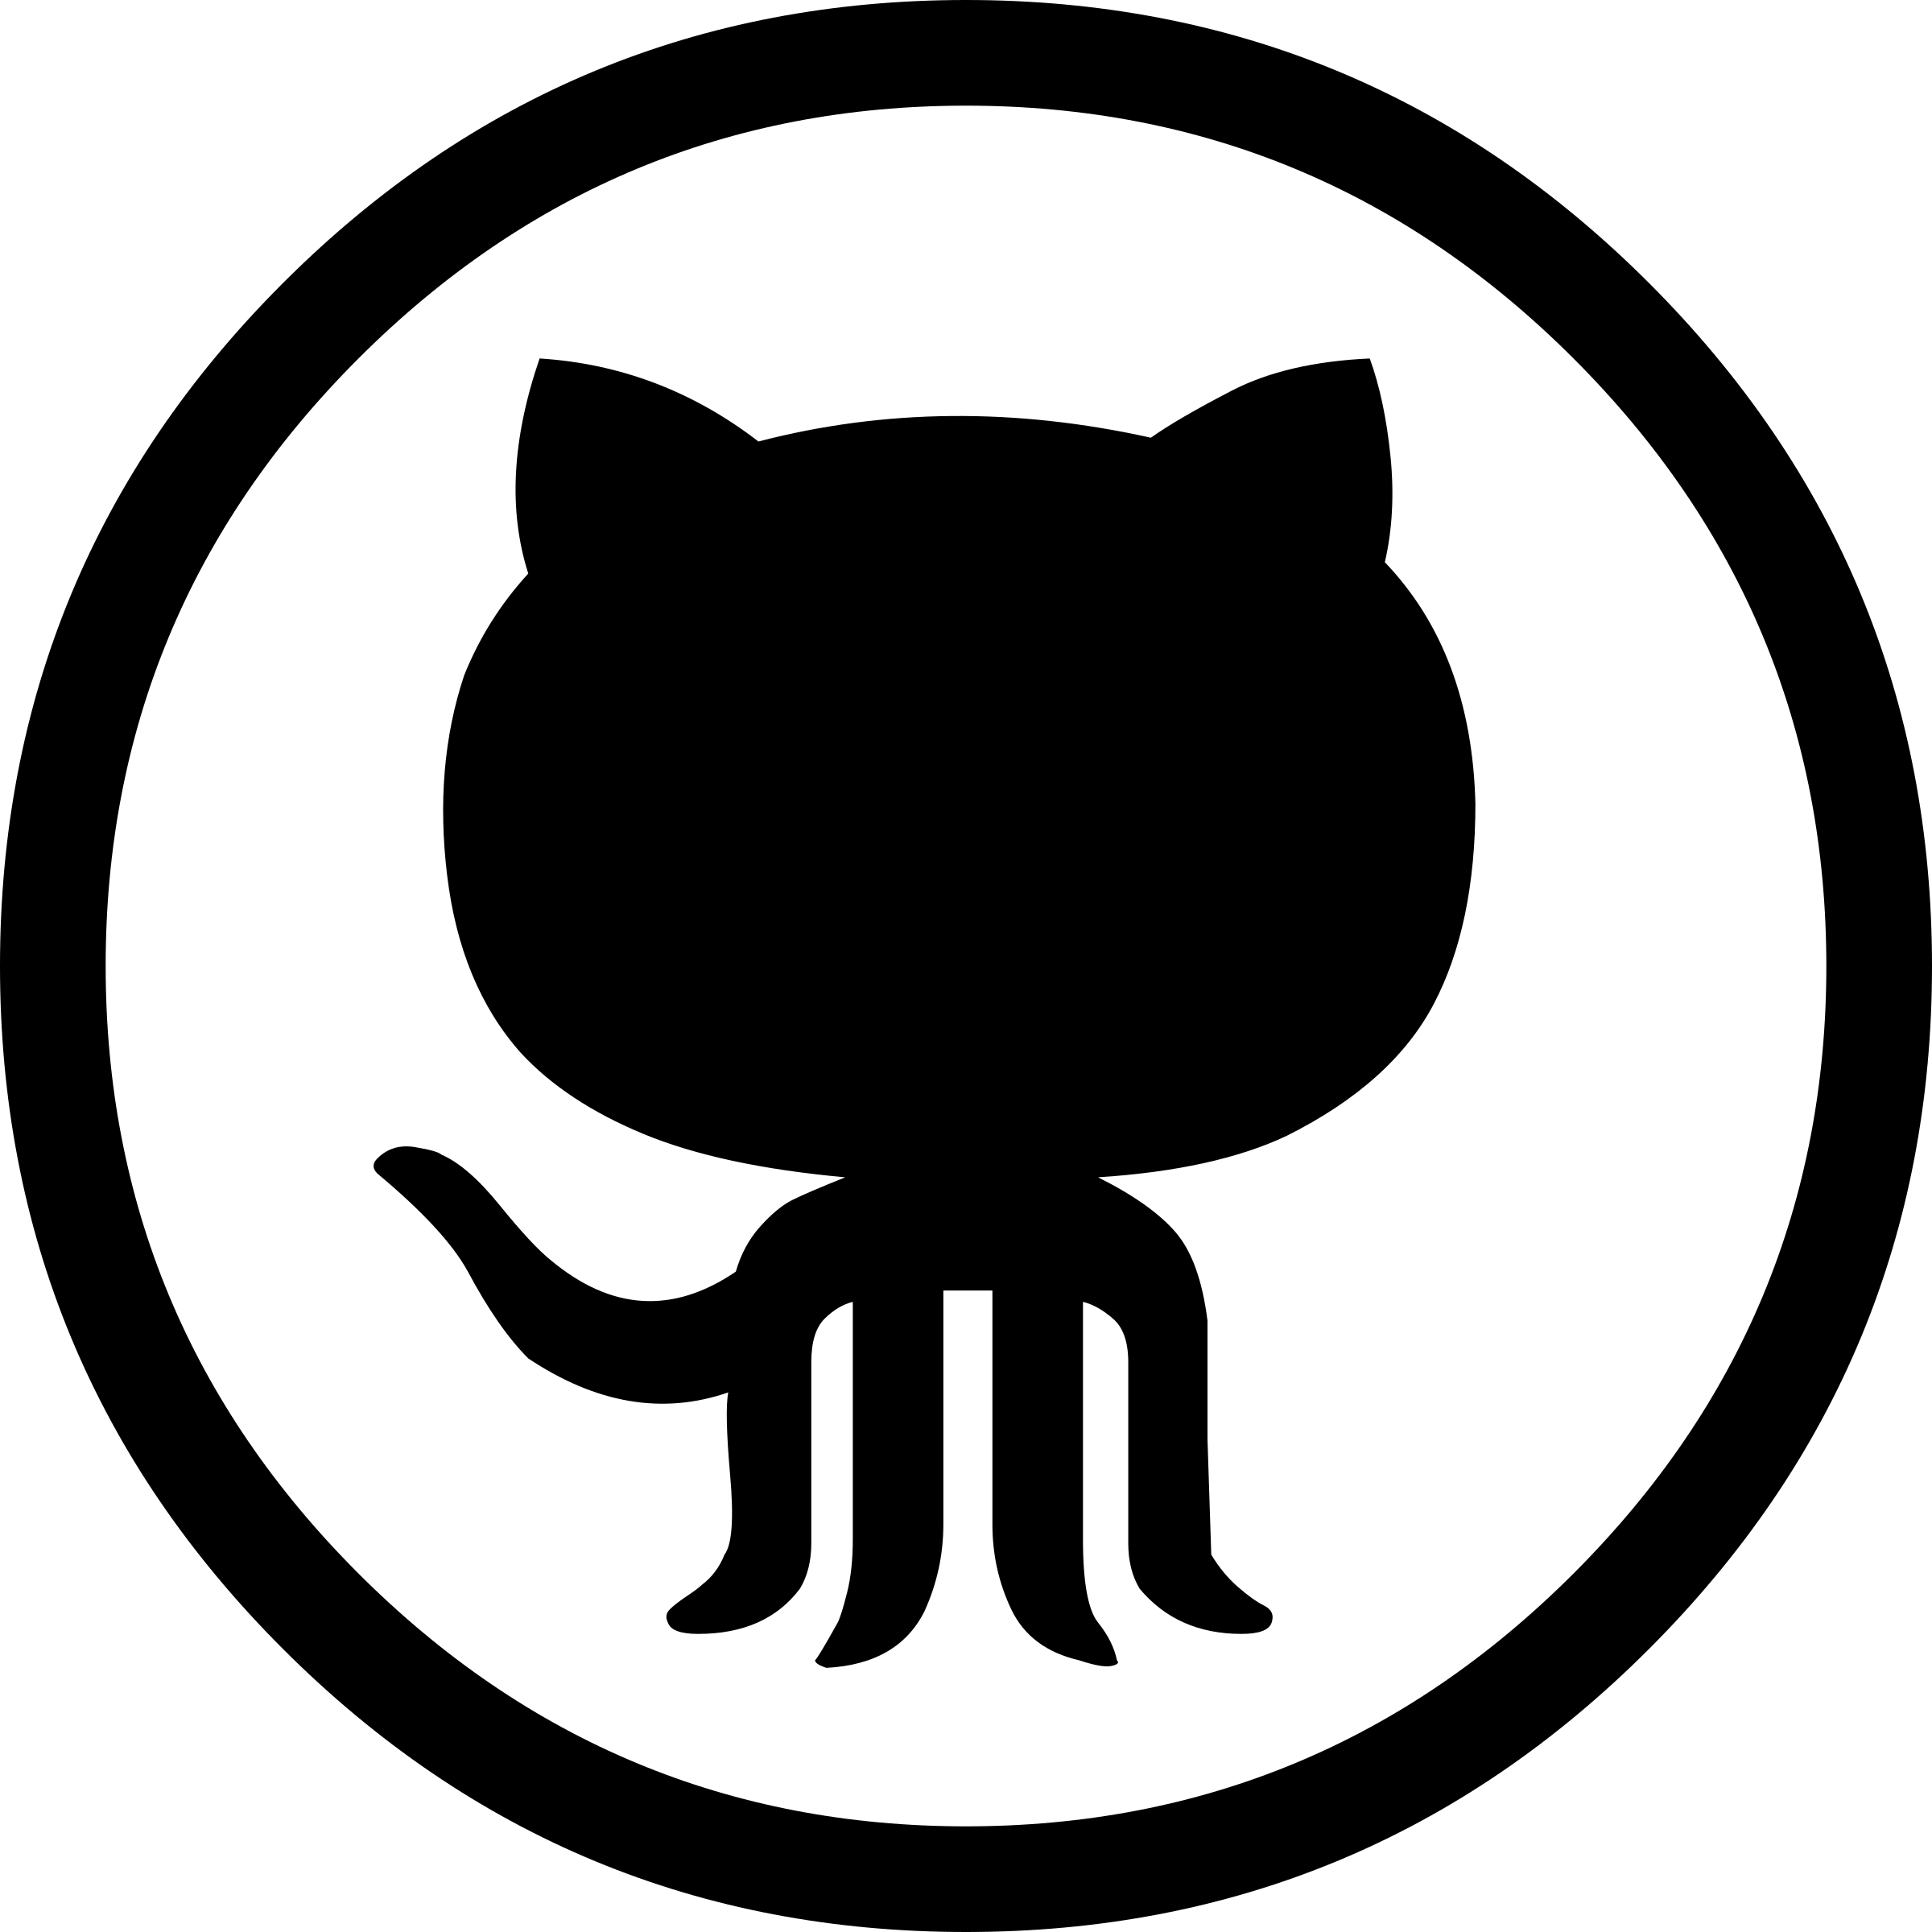
\includegraphics[width=80pt]{images/github.png}\\
  \end{center}
\end{frame}
\section{Introdução}
\begin{frame}
  \frametitle{Internet of Things}
  \begin{center}
    \includegraphics[width=270pt]{images/iot.png}\\
  \end{center}
\end{frame}

\begin{frame}
  \frametitle{Sistemas embarcados}
   \begin{center}
    \includegraphics[width=270pt]{images/embedded.png}\\
     \vspace{10pt}
    \begin{columns}
      \begin{column}{0.38\textwidth}
      \begin{center}
        \textbf{Consumo}
      \end{center}
      \end{column}
      \begin{column}{0.38\textwidth}
      \begin{center}
        \textbf{Memória}
      \end{center}
      \end{column}
      \begin{column}{0.38\textwidth}
      \begin{center}
        \textbf{Conectividade}
      \end{center}
      \end{column}
    \end{columns}
  \end{center}
\end{frame}

\begin{frame}[fragile]
  \frametitle{Sinal Analógico}

  \begin{figure}[ht]
     \centering
    \label{Sinal-Analogico}
    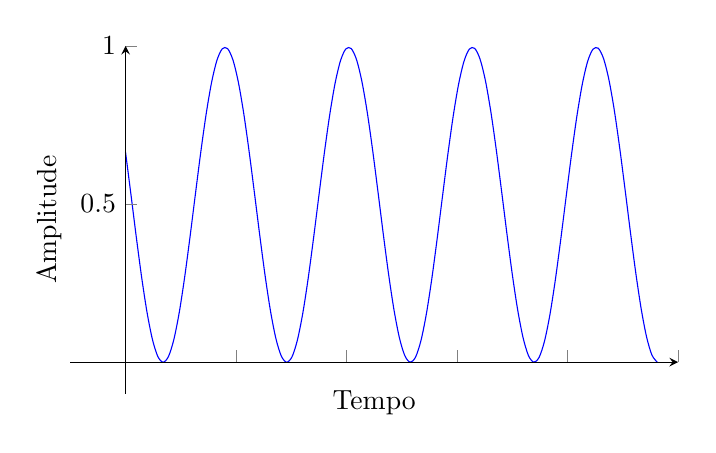
\begin{tikzpicture}
      %\draw[->] (-2,0) -- (5.3,0);
      %\draw[->] (-2,-2) -- (-2,2);
      {\draw[blue,smooth,samples=100,domain= 0.7:7.455]
      plot(\x,{2.4+2*sin(\x r*4 )});}
      \begin{axis}[
        width=9.3cm,
        height=6cm,
        x axis line style={-stealth},
        y axis line style={-stealth},
         % title={Square wave},
       xticklabels={},
       ymax = 1.2,xmax=7.5,
       axis lines*=center,
       ytick={0.5,1},
       xlabel={Tempo},
       ylabel={Amplitude},
       xlabel near ticks,
       ylabel near ticks]
     \end{axis}
   \end{tikzpicture}
   \caption{Sinal Analógico}   
  \end{figure}

\end{frame}


\begin{frame}[fragile]
\frametitle{Sinal digital}

\begin{figure}[ht]
\centering
\label{Sinal-Digital}
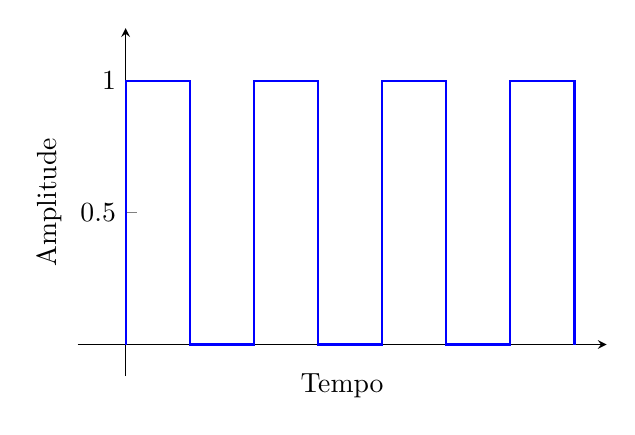
\begin{tikzpicture}
\begin{axis}[
width=8.3cm,
height=6cm,
      x axis line style={-stealth},
          y axis line style={-stealth},
             % title={Square wave},
             xticklabels={},
             ymax = 1.2,xmax=7.5,
             axis lines*=center,
             ytick={0.5,1},
             xlabel={Tempo},
             ylabel={Amplitude},
             xlabel near ticks,
             ylabel near ticks]
             \addplot+[thick,mark=none,const plot]
             coordinates
               {(0,0) (0,1) (1,0) (2,1) (3,0) (4,1) (5,0) (6,1) (7,0)};
         \end{axis}
     \end{tikzpicture}
     \caption{Sinal Digital}
  \end{figure}
\end{frame}

\begin{frame}{Descriptions}
\frametitle{Microcontrolador}
  \hfill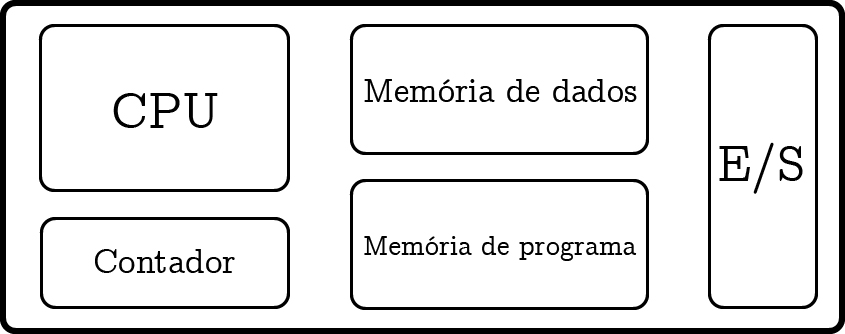
\includegraphics[width=30em]{images/Microcontrolador.jpg}\hspace*{\fill}

\end{frame}

\iffalse
\begin{frame}{Lists}
\frametitle{CPU}
  \begin{itemize}
    \item Central processing unit
    \item Executa, sequencialmente, instruções da \textbf{memória de programa}
  \end{itemize}
\end{frame}

\begin{frame}{Lists}
\frametitle{Memória}
    \begin{columns}
      \begin{column}{0.48\textwidth}
        \begin{center}
          \textbf{Memória de Programa}
            \begin{itemize}
              \item Volátil
              \item *ROM
              \item \textbf{FlashROM}
            \end{itemize}
        \end{center}
      \end{column}
      \begin{column}{0.48\textwidth}
        \begin{center}
          \textbf{Memória de Dados}
            \begin{itemize}
              \item Não-volátil
              \item RAM (Random access memory)
              \item Endereço de registradores
            \end{itemize}
        \end{center}
      \end{column}
    \end{columns}
\end{frame}
\fi

\begin{frame}{Lists}
  \frametitle{Periféricos de entrada e saída}
  \begin{center}
    \textbf{GPIOs} \\
    \textit{General purpose I/O}
    \begin{itemize}
      \item Entrada/saída
      \item Digital/analógico
      \item Interrupção
    \end{itemize}
    \includegraphics[width=230pt]{images/pins.png}\\
  \end{center}
\end{frame}

\begin{frame}{Lists}
\frametitle{Periféricos de entrada e saída}
  \begin{columns}
    \begin{column}{0.48\textwidth}
      \begin{center}
        \textbf{Sensores}
        \begin{itemize}
          \item Temperatura
          \item Inerciais (aceletômetro, etc.)
          \item Leitores (RFID, biométrico, etc.)\\
        \end{itemize}
        \vspace{30pt}
        \includegraphics[width=110pt]{images/sensors.png}\\
      \end{center}
    \end{column}
    \begin{column}{0.48\textwidth}
      \begin{center}
        \textbf{Atuadores}
        \begin{itemize}
          \item Motor
          \item Lâmpada/LED
          \item Alto-falante\\
        \end{itemize}
        \vspace{30pt}
        \includegraphics[width=110pt]{images/actuator.png}\\
      \end{center}
    \end{column}
  \end{columns}
\end{frame}

\section{ESP8266}

\begin{frame}{Summary}
  \frametitle{O que é?}
  \begin{center}
  \begin{itemize}
    \item Microcontrolador de 32-bits
    \item Modem Wi-Fi
    \item Baixo custo
    \item Comunidade ativa
  \end{itemize}
  \includegraphics[width=180pt]{images/espressif.png}\\
  \end{center}
\end{frame}

\begin{frame}{Modelos}
  \frametitle{Modelos}
  \begin{center}
    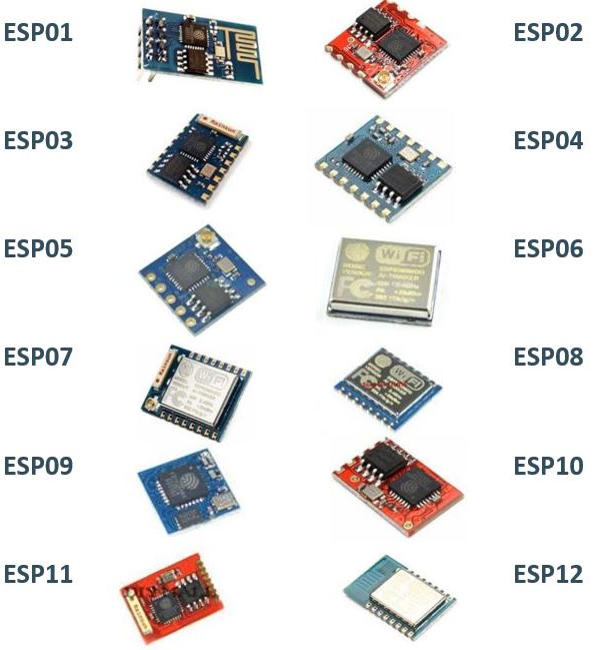
\includegraphics[width=200pt]{images/esps.png}\\
  \end{center}
\end{frame}

\begin{frame}{Animation}
  \frametitle{Especificações}
  \begin{table}[]
    \begin{tabular}{|l|l|l|}
      \hline
     & ESP-12           & ATMEGA-328p     \\ \hline
     Arquitetura                                                      & 32-bits          & 8-bits          \\ \hline
     Frequência                                                       & 80 $\sim$160 MHz & 16 $\sim$20 MHz \\ \hline
     \begin{tabular}[c]{@{}l@{}}Tensão \\ \\ de operação\end{tabular} & 2.5 $\sim$3.6V   & 1.8 $\sim$5.5V  \\ \hline
       \begin{tabular}[c]{@{}l@{}}Memória \\ \\ Flash\end{tabular}      & 1Mb $\sim$4Mb    & 32Kb            \\ \hline
       \begin{tabular}[c]{@{}l@{}}Memória \\ \\ RAM\end{tabular}      & 15 $\sim$26Kb*    & 2Kb            \\ \hline
         GPIOS                                                            & 18 (17/d e 1/a)  & 20 (14/d e 6/a) \\ \hline
         Preço                                                            & \$8,79           & \$9,99          \\ \hline
\end{tabular}
  \end{table}
\end{frame}

\begin{frame}{Comunicação}
  \frametitle{Comunicação}
  SPI
  \begin{center}
  
  \includegraphics[width=130pt]{images/SPI.png}\\
 \end{center}
  UART
 \begin{center}
  \includegraphics[width=130pt]{images/uart.png}\\
 \end{center}
  I2C
 \begin{center}
  \includegraphics[width=130pt]{images/i2c.png}\\
 \end{center}
\end{frame}

\begin{frame}{Figures}
  \frametitle{Wi-Fi}
  \begin{columns}
    \begin{column}{0.48\textwidth}
      \begin{center}
        \textbf{STA}\\
        \textit{Station}\\
        \vspace{30pt}
        \includegraphics[width=130pt]{images/sta.png}\\
      \end{center}
    \end{column}
    \begin{column}{0.48\textwidth}
      \begin{center}
        \textbf{AP}\\
        \textit{Access point}\\
        \vspace{30pt}
        \includegraphics[width=130pt]{images/ap.png}\\
      \end{center}
    \end{column}
  \end{columns}
\end{frame}

\begin{frame}{Consumo de Energia}
  \frametitle{Consumo de Energia}

    \begin{columns}
      \begin{column}{0.38\textwidth}
        \begin{center}
          \textbf{Modem sleep}
            \begin{itemize}
              \item Suspensão do modem Wi-Fi
              \item 15mA
            \end{itemize}
        \end{center}
      \end{column}
      \begin{column}{0.38\textwidth}
        \begin{center}
          \textbf{Light sleep}
            \begin{itemize}
              \item Suspensão do modem Wi-Fi e CPU
              \item 0.9mA
            \end{itemize}
        \end{center}
      \end{column}
      \begin{column}{0.38\textwidth}
        \begin{center}
          \textbf{Deep sleep}
            \begin{itemize}
              \item Desabilitação do Wi-Fi e suspensão da CPU
              \item 20$\mu$A
            \end{itemize}
        \end{center}
      \end{column}
    \end{columns}
    \begin{center}
      \vspace{20pt}
      \includegraphics[width=170pt]{images/power.png}\\
    \end{center}
\end{frame}

\begin{frame}{Tipos de boot}
  \frametitle{Tipos de boot}
    \begin{columns}
      \begin{column}{0.38\textwidth}
        \begin{center}
          \textbf{Flash Mode}
            \begin{itemize}
              \item 'Boota' pela FlashROM
            \end{itemize}
        \end{center}
      \end{column}
      \begin{column}{0.38\textwidth}
        \begin{center}
          \textbf{UART Mode}
            \begin{itemize}
              \item Não 'boota' pela FlashROM
              \item Aguarda comunicação pela UART (TX/RX)
            \end{itemize}
        \end{center}
      \end{column}
      \begin{column}{0.38\textwidth}
        \begin{center}
          \textbf{SDIO Mode}
            \begin{itemize}
              \item 'Boota' pelo cartão SD
            \end{itemize}
        \end{center}
      \end{column}
    \end{columns}
    \vspace{40pt}
    \includegraphics[width=300pt]{images/boot-table.png}\\
\end{frame}

\begin{frame}{Software}
  \frametitle{Software}
  \begin{columns}
        \begin{column}{0.48\textwidth}
          \begin{center}
            
\includegraphics[width=80pt]{images/nodemcu.png}\\
            \textbf{NodeMCU firmware}\\
            \textit{Lua}\\
            \begin{itemize}
              \item Linguagem interpretada
              \item Padrão das placas NodeMCU
              \item Comunidade média
            \end{itemize}
          \end{center}


        \end{column}
        \begin{column}{0.48\textwidth}
          \begin{center}
            
\includegraphics[height=80pt]{images/arduino.png}\\
            \textbf{Arduino core firmware}\\
            \textit{Arduino/C++}\\
            \begin{itemize}
              \item Linguagem compilada
              \item Utilização da Arduino IDE
              \item Comunidade gigante
            \end{itemize}
          \end{center}
        \end{column}
  \end{columns}

\end{frame}

\begin{frame}{Software}
  \frametitle{Software}
    \begin{center}
      
\includegraphics[width=120pt]{images/micropython.png}\\
      \textbf{Micropython}\\
      \textit{Python}\\
      \begin{itemize}
        \item Linguagem interpretada
        \item Linguagem acessível a iniciantes e poderosa para experientes
        \item Comunidade gigante
        \item \textit{upip} (versão micro do \textit{pip})
        \item Otimização da memória RAM (???)
      \end{itemize}
    \end{center}
\end{frame}

\begin{frame}{Micropython - Otimização da RAM}
  \frametitle{Micropython - Otimização da RAM}
  \begin{columns}
    \begin{column}{0.48\textwidth}
      \begin{center}
        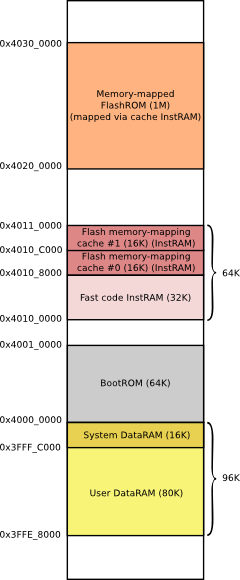
\includegraphics[width=95pt]{images/mem-mapping.png}\\
      \end{center}
    \end{column}
    \begin{column}{0.48\textwidth}
      \begin{center}
        \begin{enumerate}
          \item Limitação da \textbf{InstRAM} \vspace{5pt}
          \item \textbf{BootRAM} possui uma biblioteca para rotinas de suporte\vspace{5pt}
          \item Essa biblioteca pode substituir instruções presentes na \textbf{InstRAM}\vspace{5pt}
          \item Aparição de \textbf{bugs}\vspace{5pt}
          \item \textbf{Micropython} faz bom uso disso e possui um Test coverage de \textbf{92\%}\vspace{5pt}
        \end{enumerate}
      \end{center}
    \end{column}
  \end{columns}
\end{frame}

\begin{frame}
  \frametitle{Micropython - Instalação e Primeiros passos}
  Instruções sobre instalação, bem como a preparação do ambiente, ferramentas, dicas, exemplos e documentação externa estão disponíveis no próprio repositório remoto do material: \\\\
  \begin{center}
    https://github.com/GabrielMMelo/esp8266\_course
  \end{center}
\end{frame}

\begin{frame}{SPIFFS}
  \frametitle{Micropython - Sistema de arquivos}

  \begin{itemize}
    \item Scripts de execução
    \item Conteúdo para um Web Server
    \item Arquivos de configuração
    \item Banco de dados


  \end{itemize}
 
  \begin{columns}
    \begin{column}{0.48\textwidth}

    \textbf{boot.py} \\
    Script executado no boot do dispositivo \\
    (possui configurações iniciais da placa, principalmente sobre comunicação)

    \end{column}
    \begin{column}{0.48\textwidth}

    \textbf{main.py} \\
    Script executado após boot.py \\
    (inicializa a árvore de execução do projeto)

    \end{column}
  \end{columns}
\end{frame}


\section{Aplicações}

\begin{frame}{Transmissão de informação por HTTP}
  \frametitle{Transmissão de informação por HTTP}
  \begin{center}
    \includegraphics[width=190pt]{images/HTTP.png}\\
  \end{center}
\end{frame}

\begin{frame}{Sistema de ponto}
  \frametitle{Sistema de ponto}
    \begin{columns}
      \begin{column}{0.48\textwidth}
        \begin{center}
          \includegraphics[width=80pt]{images/rfid.png}\\
          \vspace{20pt}
          \textbf{RFID}
       \end{center}
      \end{column}
      \begin{column}{0.48\textwidth}
        \vspace{-60pt}
        \begin{center}
          \includegraphics[width=150pt]{images/card-ufla.png}\\
          \textbf{Cartão universitário}
        \end{center}
      \end{column}
    \end{columns}

 \vspace{40pt}
 * https://github.com/wendlers/micropython-mfrc522
\end{frame}

\begin{frame}{Sistema de controle residencial}
  \frametitle{Sistema de controle residencial}

    \hfill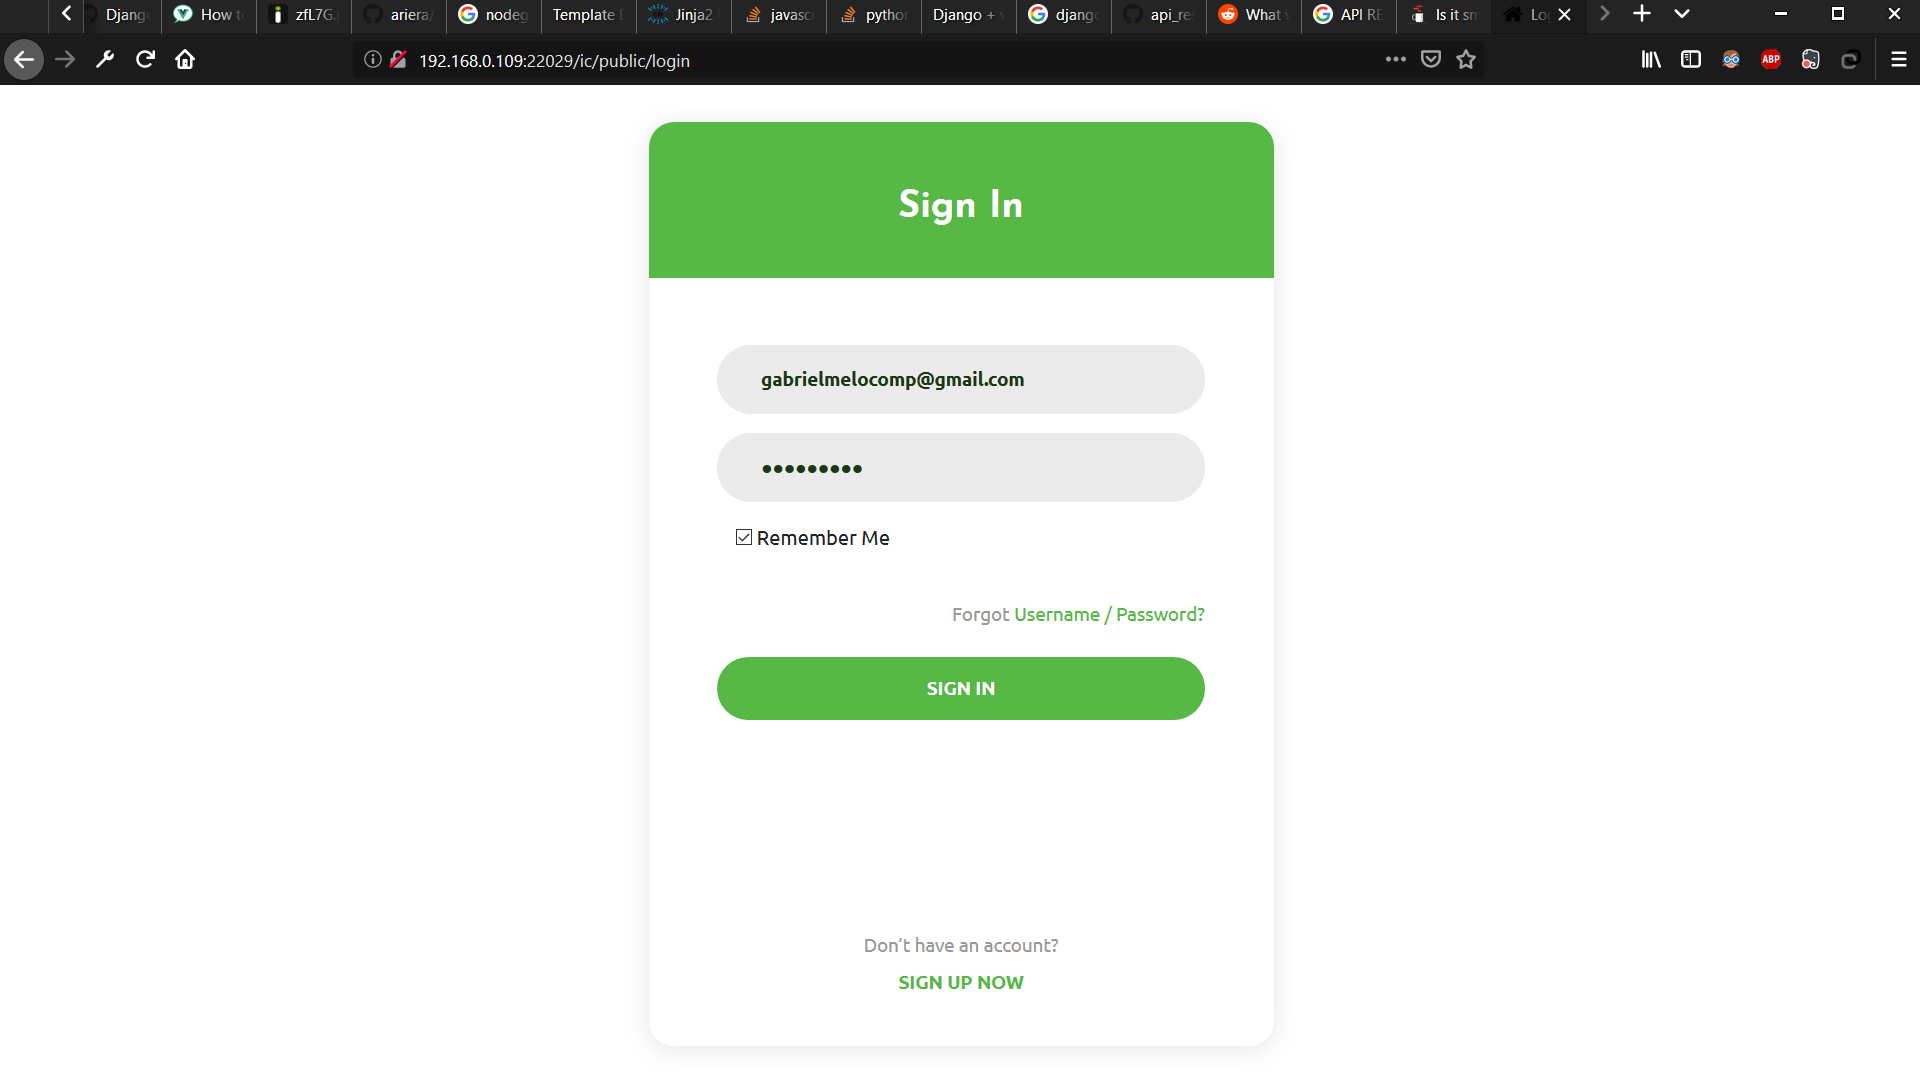
\includegraphics[width=300pt]{images/iot-server_login.png}\hspace*{\fill}
\end{frame}

\begin{frame}{Sistema de controle residencial}
  \frametitle{Sistema de controle residencial}
  \begin{center}
    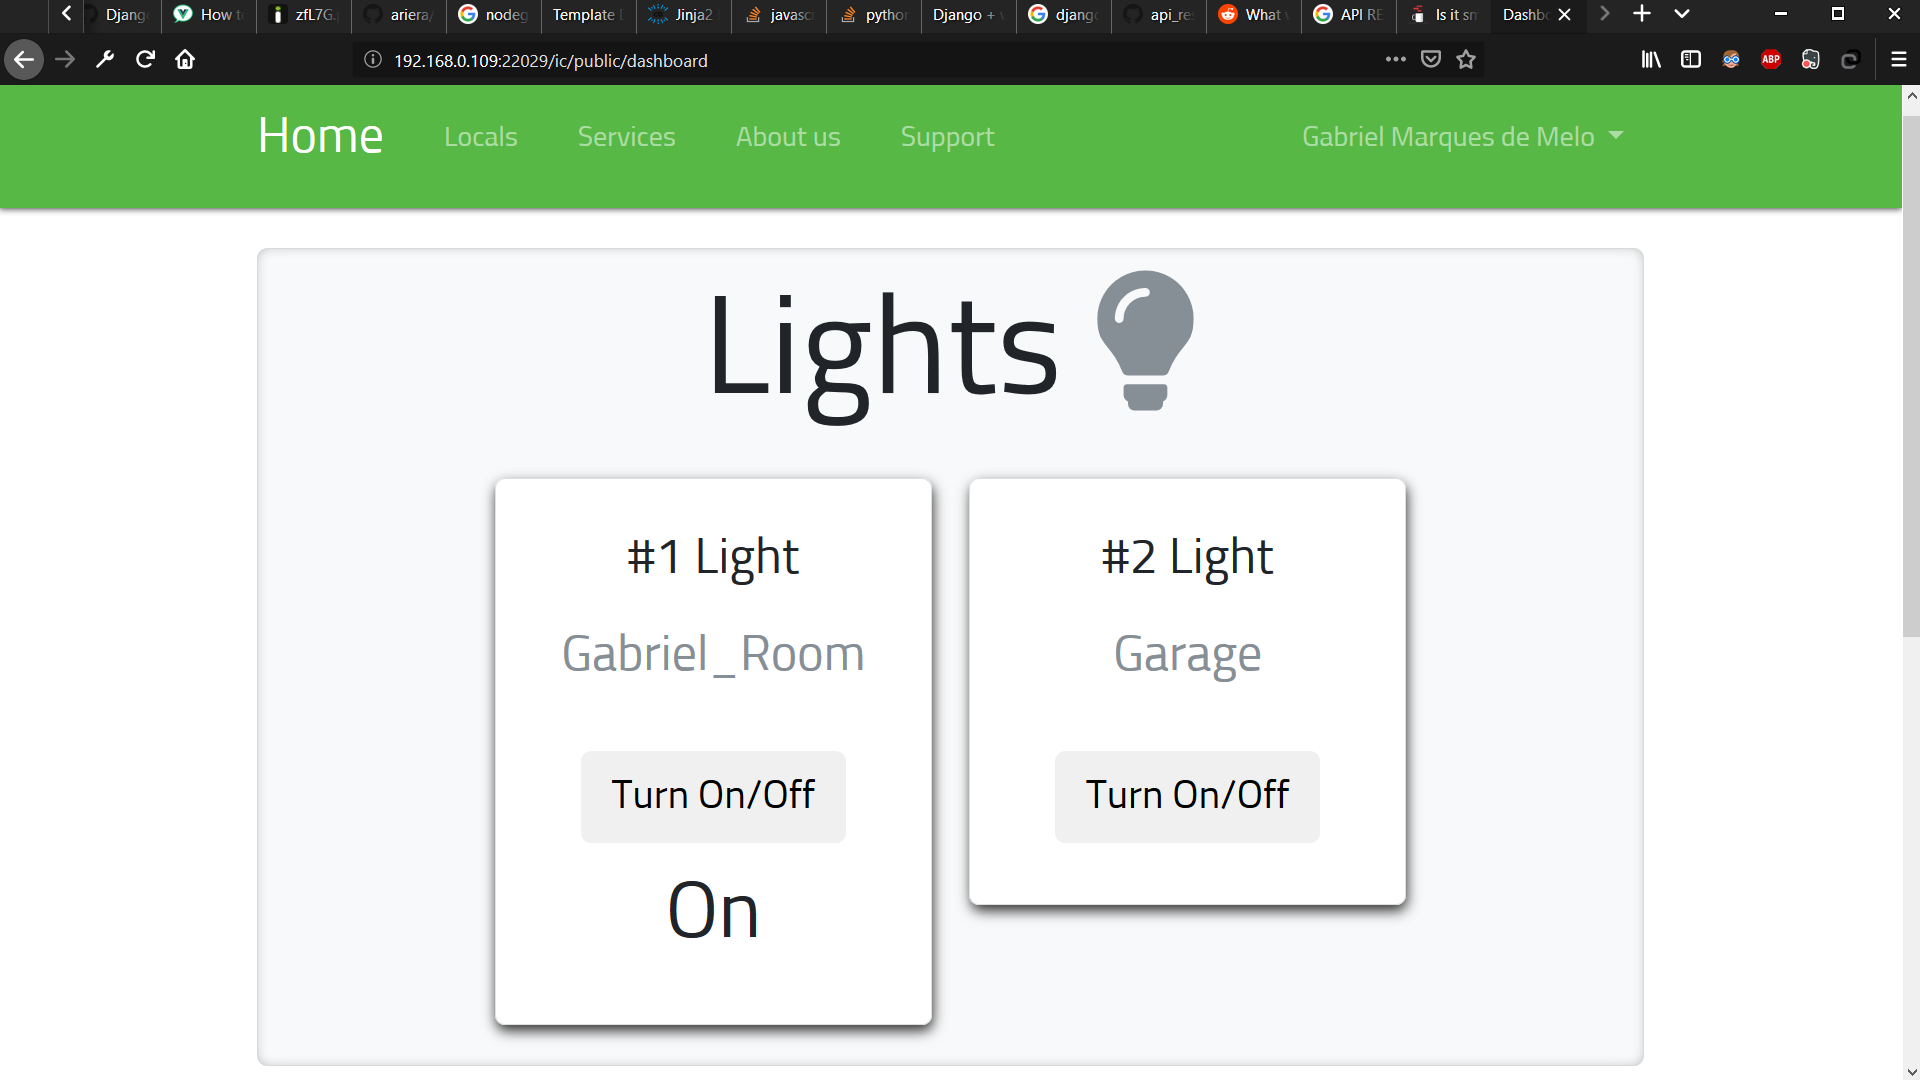
\includegraphics[width=300pt]{images/iot-server_dash1.png}
  \end{center}
\end{frame}

\begin{frame}{Sistema de controle residencial}
  \frametitle{Sistema de controle residencial}
  \begin{center}
    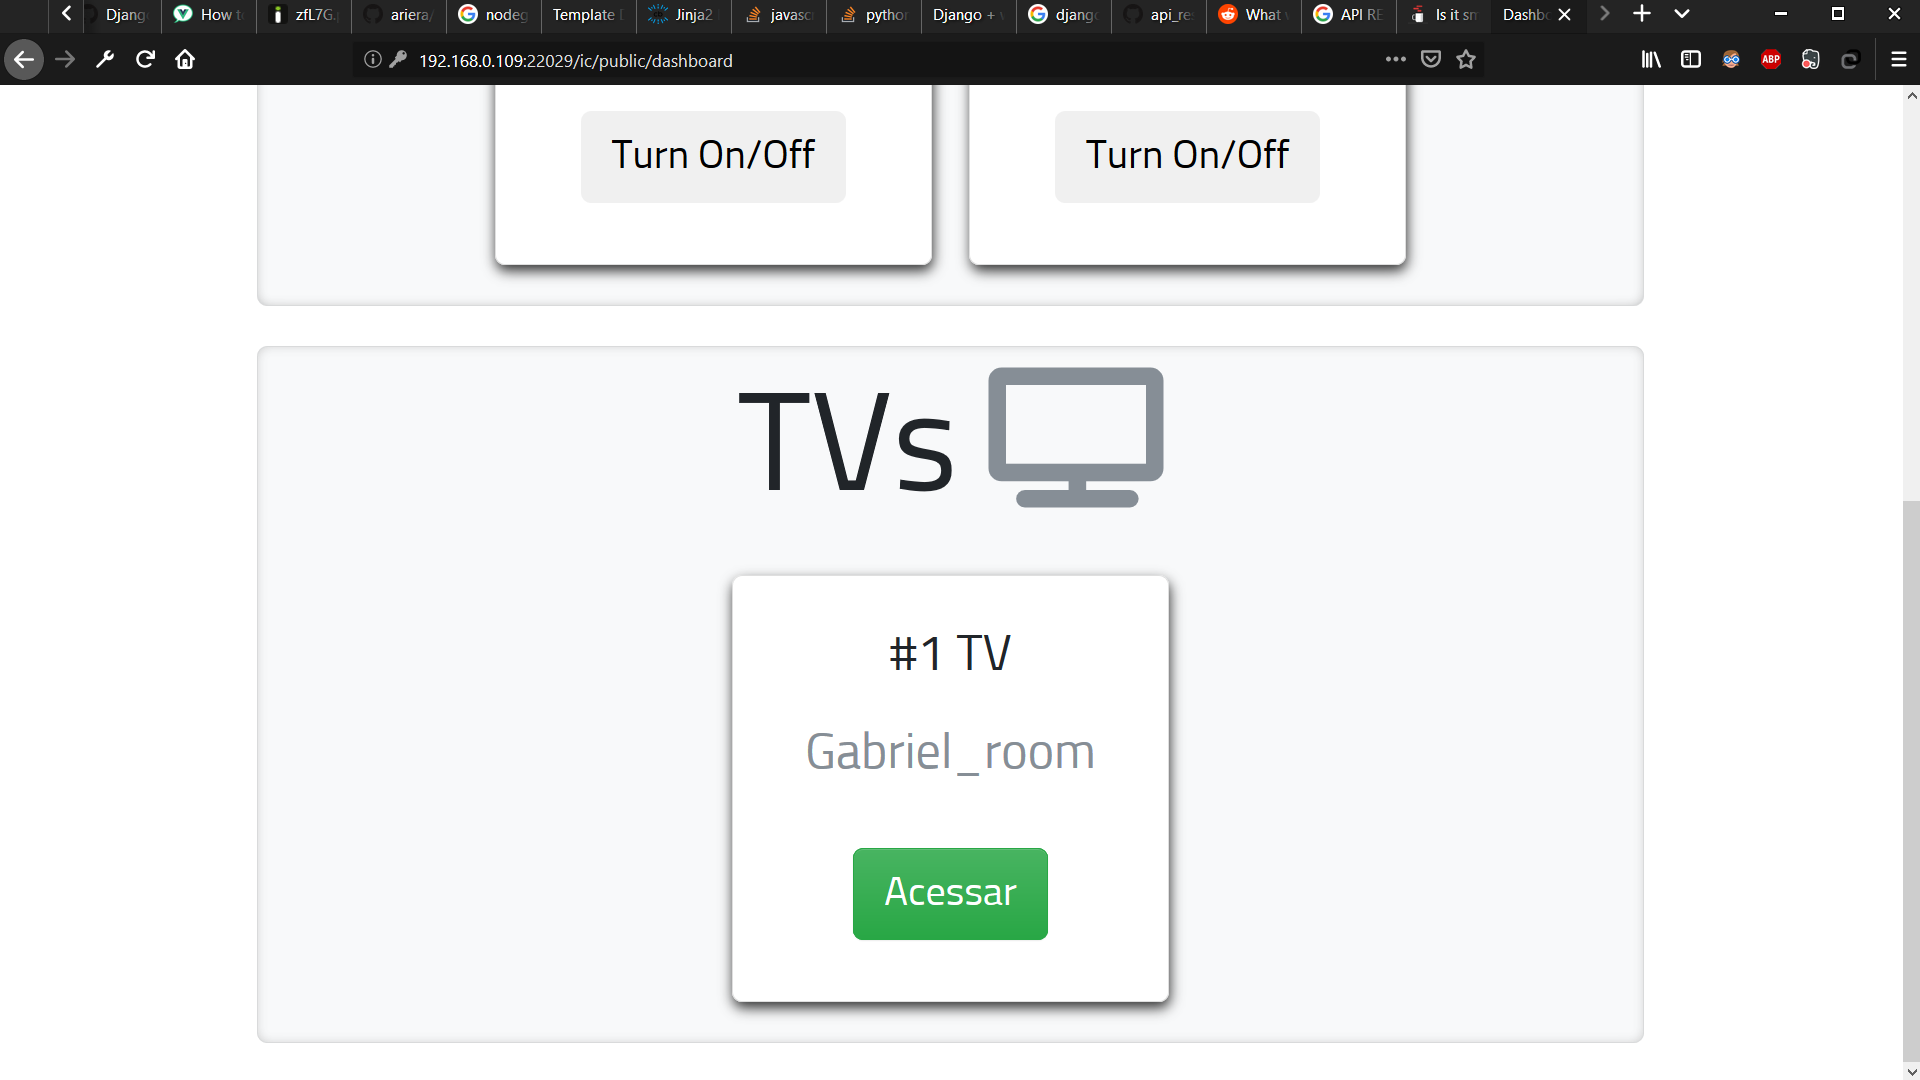
\includegraphics[width=300pt]{images/iot-server_dash2.png}
  \end{center}
\end{frame}

\begin{frame}{Sistema de controle residencial}
  \frametitle{Sistema de controle residencial}
  \begin{center}
    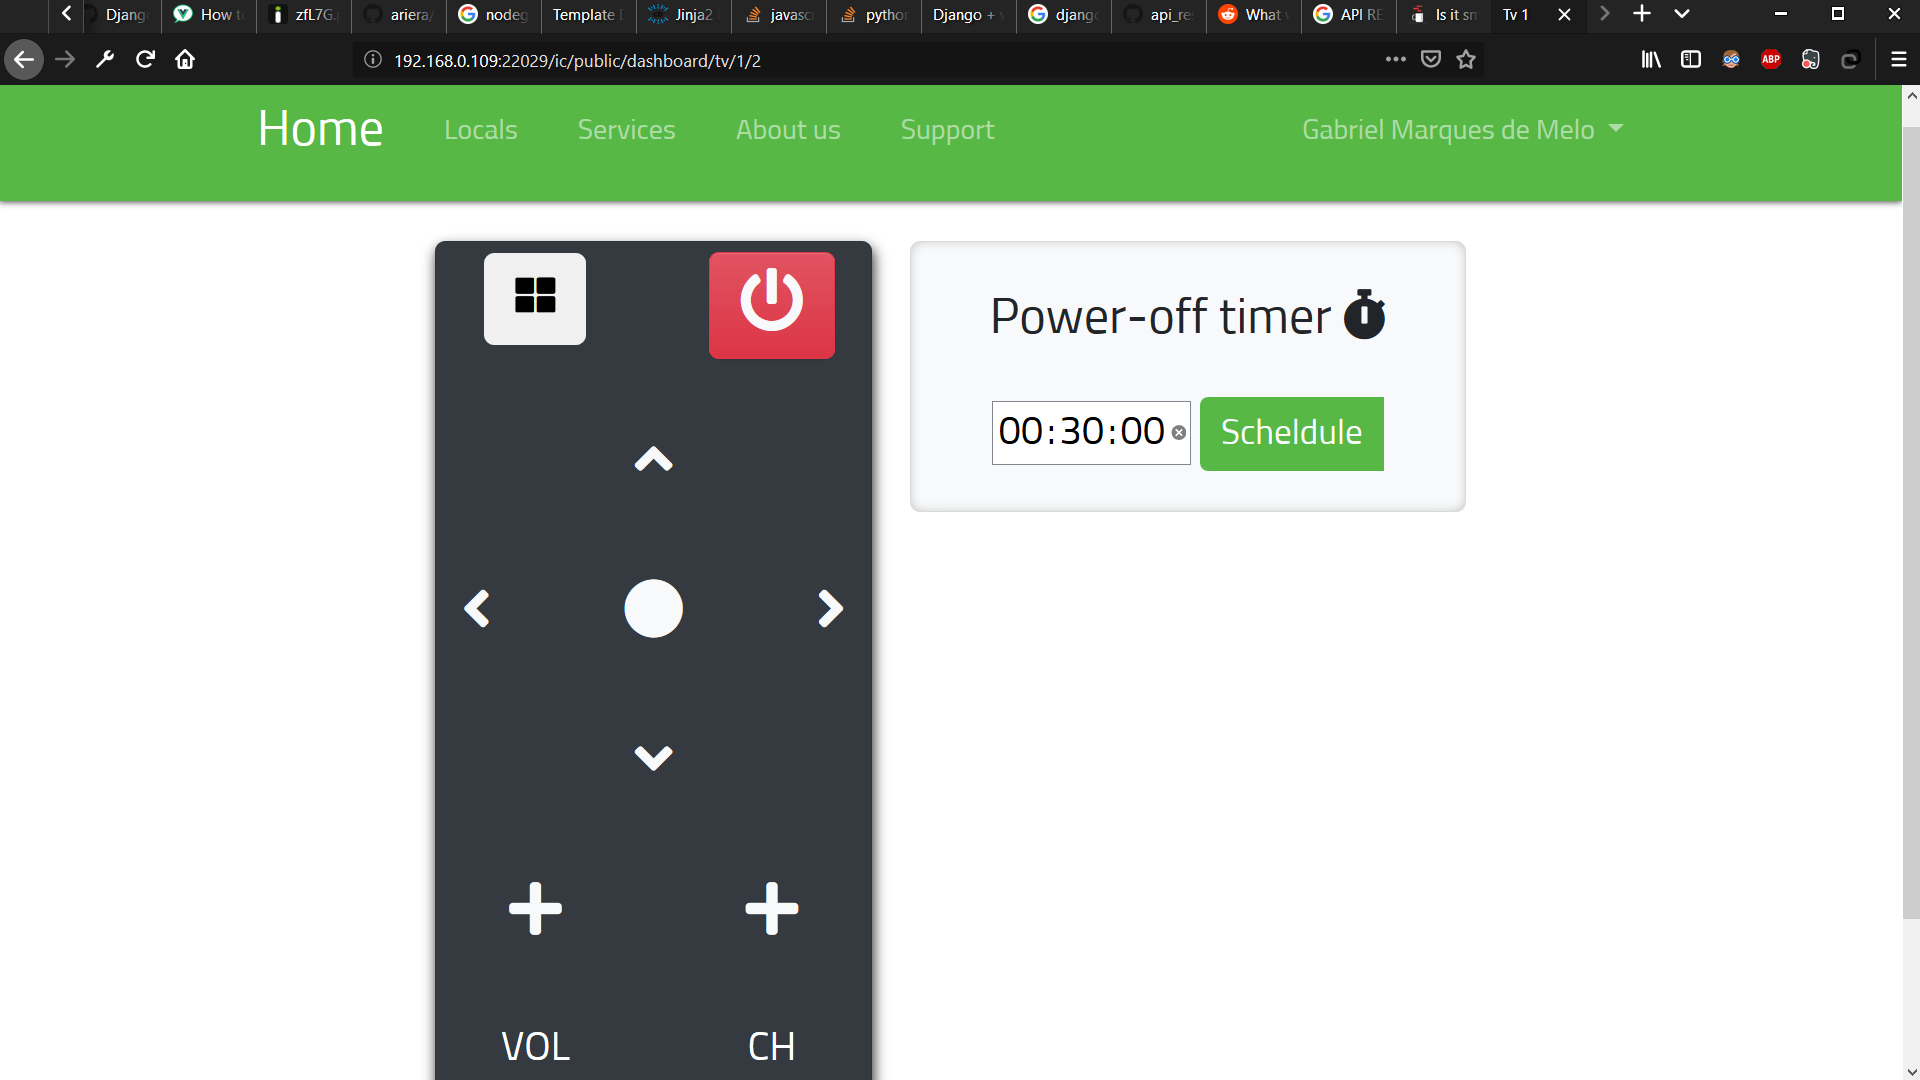
\includegraphics[width=300pt]{images/iot-server_remotecontrol.png}
  \end{center}
\end{frame}
\section{Extras}

\begin{frame}{Summary}
  \frametitle{esp-open-sdk}
  \vspace{15pt}
  \begin{itemize}
    \item Software development kit para ESP8266
    \item Acesso as instruções da Xtensa lx106
    \item Programação em C e assembly
    \item \href{https://github.com/pfalcon/esp-open-sdk}{Projeto no GitHub}
    \item *\href{https://github.com/SuperHouse/esp-open-rtos}{Complemento usando rtos}
  \end{itemize}
\end{frame}

\begin{frame}{ESP32}
  \frametitle{ESP32}
  \vspace{15pt}
  \begin{itemize}
    \item Dual-core
    \item Wi-Fi + Bluetooth 4.0
    \item 240MHz
  \end{itemize}

  \begin{center}
    \includegraphics[width=200pt]{images/esp32.png}\\
  \end{center}
\end{frame}

\section{Referências}

\begin{frame}{Summary}
  \frametitle{Referências}
  \vspace{15pt}
  \begin{itemize}
    \item \textbf{ESP8266: Uma introdução ao IoT}, disponível em: https://github.com/GabrielMMelo/esp8266\_course \vspace{15pt}
    \item \textbf{Documentação Micropython}: https://docs.micropython.org/en/latest/esp8266/tutorial/intro.html \vspace{5pt}
    \item \textbf{Pacotes upip} (nem todos possuem suporte para port ESP8266): https://pypi.org/search/?q=micropython- \vspace{15pt}
    \item \textbf{Discussão acerca do uso do Micropython com ESP8266}: https://www.kickstarter.com/projects/214379695/micropython-on-the-esp8266-beautifully-easy-iot/posts/1501224 \vspace{5pt}
  \end{itemize}
\end{frame}



\plain{}{Perguntas?}

\end{document}
